For both the Venturi and Orifice meter we choose 6 values of $Q$ and measure $P_d$, $P_v$ and $\Delta p$ as seen in fig \ref{fig:setup}

\begin{figure}[h!]
  \begin{subfigure}{0.51\columnwidth}
    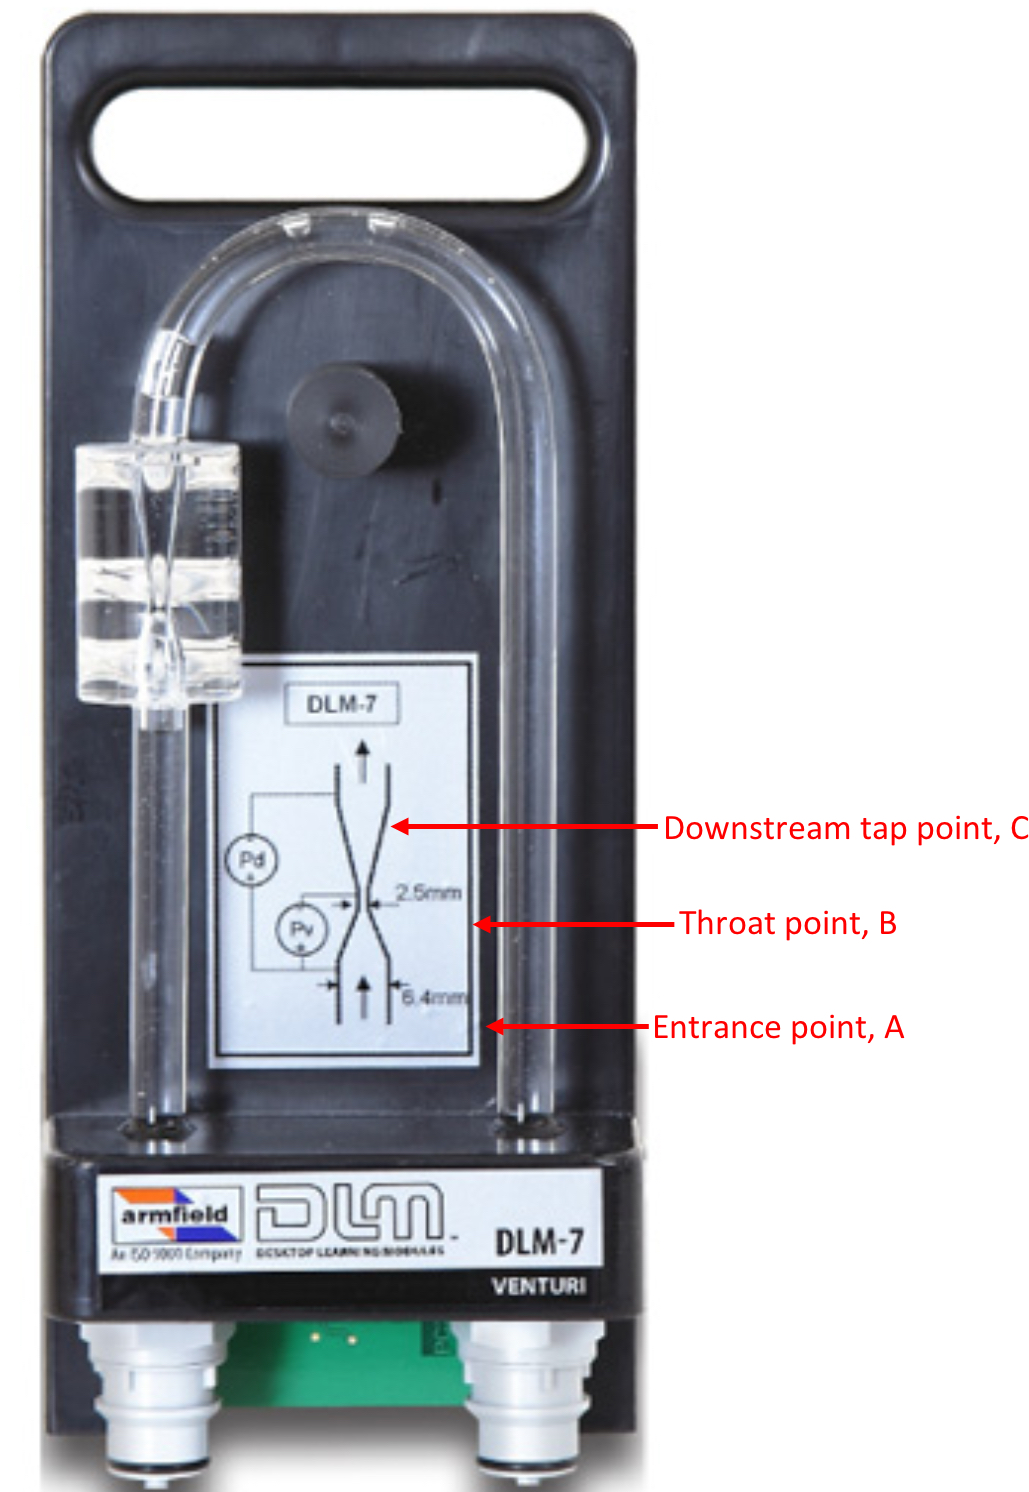
\includegraphics[width=\linewidth]{Diagrams/Venturi.jpeg}
    \caption{Venturi meter} 
    \label{fig:Venturi}
  \end{subfigure}%
  \hspace*{\fill}   % maximize separation between the subfigures
  \begin{subfigure}{0.435\columnwidth}
    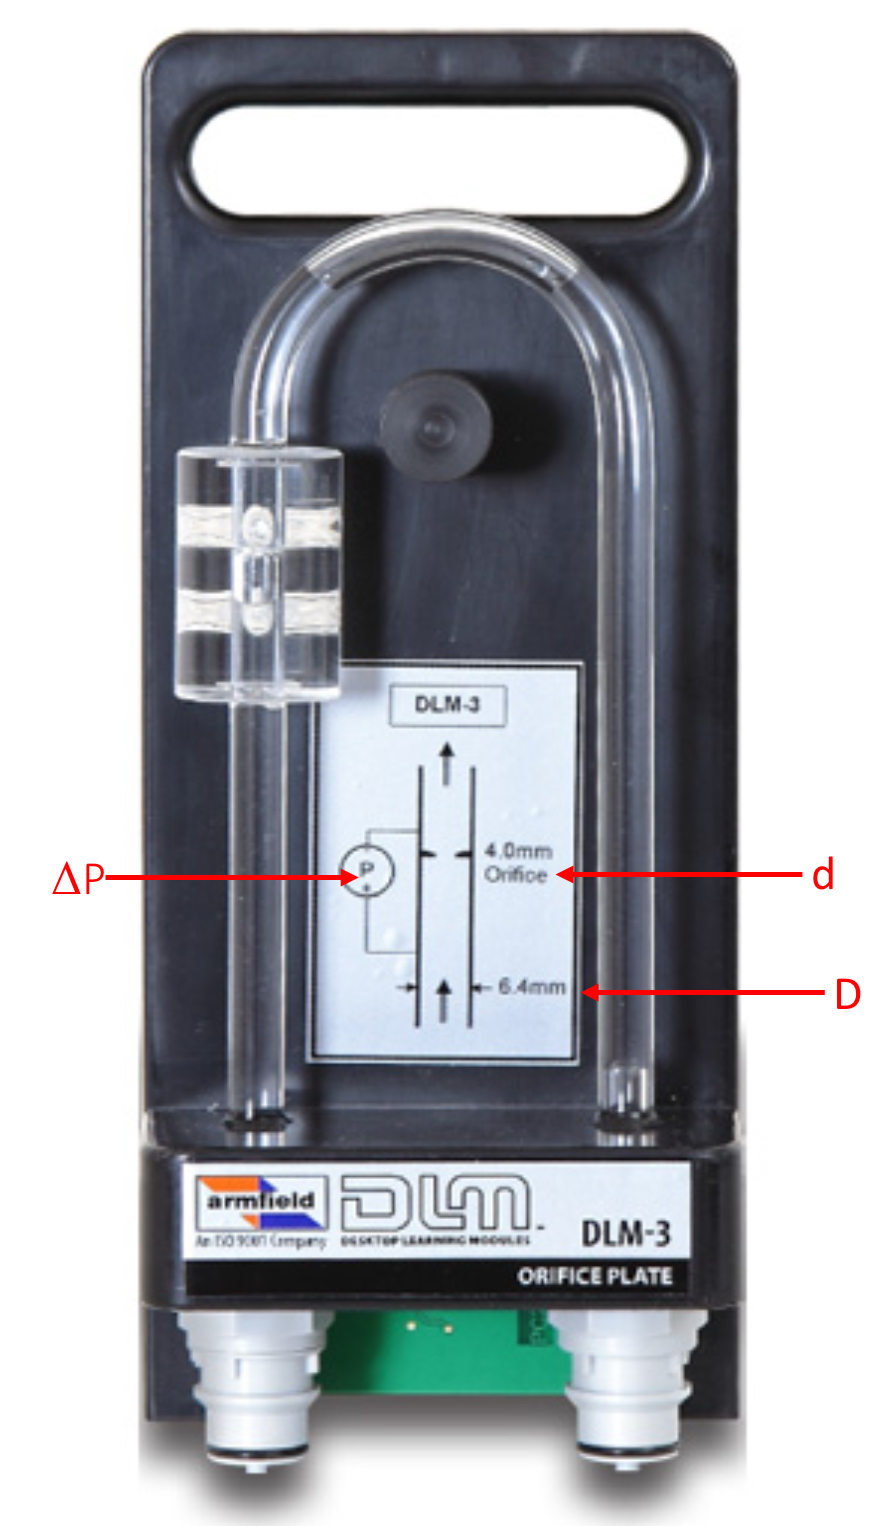
\includegraphics[width=\linewidth]{Diagrams/Orifice.jpeg}
    \caption{Orifice meter} 
    \label{fig:Orifice}
  \end{subfigure}%

\label{fig:setup}
\caption{Overview of the two different systems in use} \label{fig:Meters}
\end{figure}
